\section{Une bague en argent (4 points)}\label{ex:bague}

Florent observe la bague de Suzanne. Suzanne lui affirme que c'est une bague en argent mais Florent pense qu'elle est en fer-blanc. Pour en avoir le c\oe ur net, il pèse la bague et trouve $m = \num{14.4} \ g$. Il plonge la bague dans une éprouvette contenant$ \num{5.0} \ mL$ d'eau : le niveau monte jusqu'à $\num{6.4} \ mL$.  

\begin{questions}
	\question[1] De combien le volume d'eau dans l'éprouvette a-t-il augmenté ? En déduire la volume de la bague de Suzanne.
	\begin{solution}
		Le volume d'eau a augmenté de $\num{1.4} mL$, donc la bague a un volume de $\num{1.4} mL$, soit $\num{1.4} cm^3.$
	\end{solution}
	
	\question[1] A l'aide des données du tableau, calculer la masse que ferait la bague si elle était en fer-blanc.
	\begin{solution}
		\begin{equation*}
		\num{1.4} \times \num{8} = \num{11,2} 
		\end{equation*}
		
		Si elle était en argent la bague aurait une masse de $\num{11,2} g$. 
	\end{solution}
	
	\question[1] A l'aide du tableau, calculer la masse que ferait la bague si elle était en argent.
	\begin{solution}
		\begin{equation*}
		\num{1.4} \times \num{10.3} = \num{14,42} 
		\end{equation*}
		
		Si elle était en argent la bague aurait une masse de $\num{14,42} g$. 
	\end{solution}
	
	\question[1] Déterminer à l'aide des réponses précédentes, si la bague de Suzanne est en argent ou en fer-blanc.
	\begin{solution}
		La masse mesurée sur la balance est $\num{14,4} g$ donc la bague est argent, Suzanne a raison.
	\end{solution}

\end{questions}

\begin{center}
	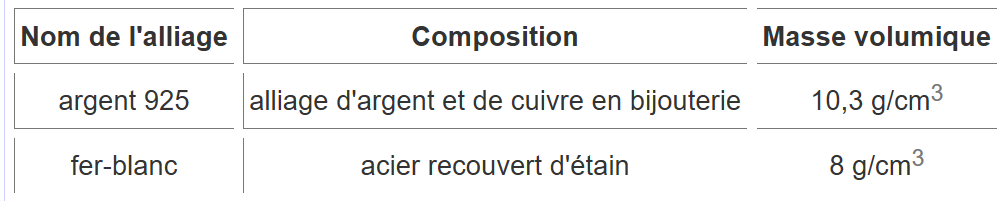
\includegraphics[scale=0.5]{img/tableau}
\end{center}
